% MCQ Generation Pipeline Diagram
% Compile with: pdflatex mcq_pipeline.tex
% Or include in main paper after loading tikz packages

\documentclass[tikz,border=8pt]{standalone}
\usepackage{tikz}
\usetikzlibrary{positioning, arrows.meta, shapes.geometric, calc}

\begin{document}

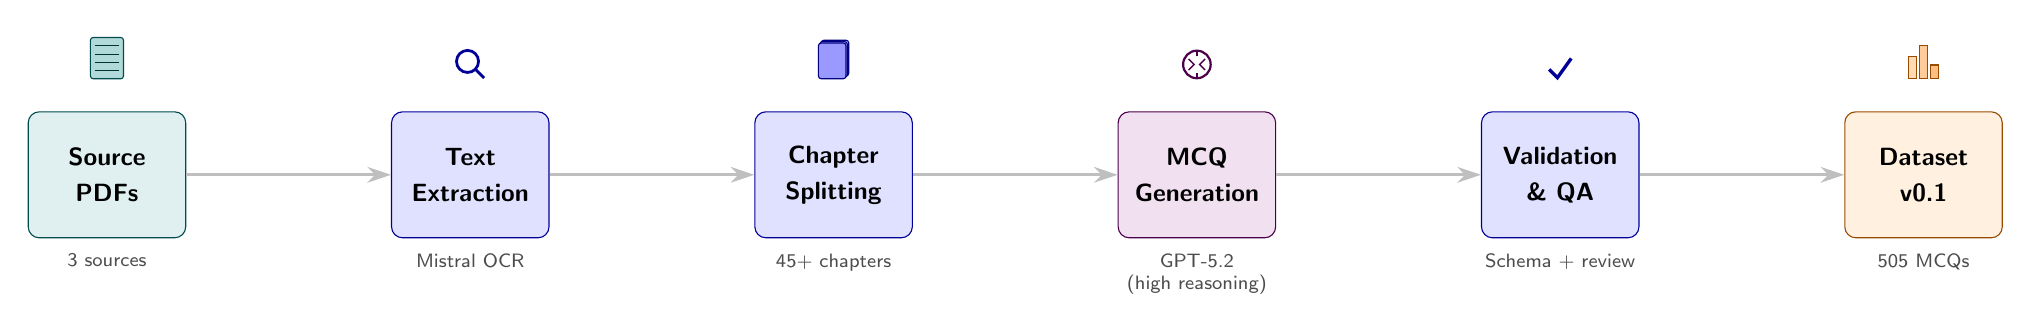
\begin{tikzpicture}[
    % Node styles
    stage/.style={
        rectangle,
        rounded corners=4pt,
        draw=#1!60!black,
        fill=#1!12,
        minimum width=2cm,
        minimum height=1.6cm,
        align=center,
        font=\small\sffamily
    },
    stage/.default=blue,
    arrow/.style={
        -{Stealth[length=3mm, width=2mm]},
        line width=1pt,
        draw=gray!50
    },
    sublabel/.style={
        font=\scriptsize\sffamily,
        text=gray!60!black
    }
]

% Define positions
\def\xsep{2.6cm}

% Stage 1: Source PDFs
\node[stage=teal] (pdf) {
    \textbf{Source}\\[2pt]
    \textbf{PDFs}
};
\node[sublabel, below=2pt of pdf] {3 sources};

% Stage 2: OCR
\node[stage, right=\xsep of pdf] (ocr) {
    \textbf{Text}\\[2pt]
    \textbf{Extraction}
};
\node[sublabel, below=2pt of ocr] {Mistral OCR};

% Stage 3: Chunking
\node[stage, right=\xsep of ocr] (chunk) {
    \textbf{Chapter}\\[2pt]
    \textbf{Splitting}
};
\node[sublabel, below=2pt of chunk] {45+ chapters};

% Stage 4: Generation
\node[stage=violet, right=\xsep of chunk] (gen) {
    \textbf{MCQ}\\[2pt]
    \textbf{Generation}
};
\node[sublabel, below=2pt of gen, align=center] {GPT-5.2\\(high reasoning)};

% Stage 5: Verification
\node[stage, right=\xsep of gen] (verify) {
    \textbf{Validation}\\[2pt]
    \textbf{\& QA}
};
\node[sublabel, below=2pt of verify] {Schema + review};

% Stage 6: Output
\node[stage=orange, right=\xsep of verify] (output) {
    \textbf{Dataset}\\[2pt]
    \textbf{v0.1}
};
\node[sublabel, below=2pt of output] {505 MCQs};

% Arrows
\draw[arrow] (pdf) -- (ocr);
\draw[arrow] (ocr) -- (chunk);
\draw[arrow] (chunk) -- (gen);
\draw[arrow] (gen) -- (verify);
\draw[arrow] (verify) -- (output);

% Icons (simple TikZ shapes)
\begin{scope}[yshift=0.5cm]
    % PDF icon
    \node[above=8pt of pdf] {
        \tikz[scale=0.35]{
            \draw[fill=teal!30, draw=teal!60!black, rounded corners=1pt] (0,0) rectangle (1.2,1.5);
            \foreach \y in {0.3, 0.6, 0.9, 1.2} {
                \draw[teal!40!black, line width=0.3pt] (0.15,\y) -- (1.05,\y);
            }
        }
    };

    % OCR icon (magnifying glass)
    \node[above=8pt of ocr] {
        \tikz[scale=0.35]{
            \draw[blue!60!black, line width=1pt] (0.5,0.5) circle (0.4);
            \draw[blue!60!black, line width=1pt] (0.78,0.22) -- (1.1,-0.1);
        }
    };

    % Chapter icon (stacked pages)
    \node[above=8pt of chunk] {
        \tikz[scale=0.35]{
            \draw[fill=blue!20, draw=blue!50!black, rounded corners=1pt] (0.1,0.1) rectangle (1.1,1.4);
            \draw[fill=blue!30, draw=blue!50!black, rounded corners=1pt] (0.05,0.05) rectangle (1.05,1.35);
            \draw[fill=blue!40, draw=blue!50!black, rounded corners=1pt] (0,0) rectangle (1,1.3);
        }
    };

    % LLM icon (brain/circuit)
    \node[above=8pt of gen] {
        \tikz[scale=0.35]{
            \draw[violet!60!black, line width=0.8pt] (0.6,0.7) circle (0.5);
            \draw[violet!60!black, line width=0.5pt] (0.3,0.5) -- (0.5,0.7) -- (0.3,0.9);
            \draw[violet!60!black, line width=0.5pt] (0.9,0.5) -- (0.7,0.7) -- (0.9,0.9);
            \draw[violet!60!black, line width=0.5pt] (0.6,0.2) -- (0.6,0.4);
            \draw[violet!60!black, line width=0.5pt] (0.6,1.0) -- (0.6,1.2);
        }
    };

    % Check icon
    \node[above=8pt of verify] {
        \tikz[scale=0.35]{
            \draw[blue!60!black, line width=1.2pt] (0.2,0.6) -- (0.5,0.3) -- (1.0,1.0);
        }
    };

    % Dataset icon (chart)
    \node[above=8pt of output] {
        \tikz[scale=0.35]{
            \draw[fill=orange!30, draw=orange!60!black] (0,0) rectangle (0.3,0.8);
            \draw[fill=orange!40, draw=orange!60!black] (0.4,0) rectangle (0.7,1.2);
            \draw[fill=orange!50, draw=orange!60!black] (0.8,0) rectangle (1.1,0.5);
        }
    };
\end{scope}

\end{tikzpicture}

\end{document}
